\documentclass{presentation_template}
% To change the slides size go to EESD.cls file and edit the preamble as explained.

% ---- Add your Meta-data to the PDF (Copyrights Kinda!) ----
\hypersetup{
  pdfinfo={
    Title={Presentation: 3D finite element modeling of historical masonry walls},
    Author={Mahmoud S. Shaqfa, Katrin Beyer},
    Subject={EPFL - ENAC - EESD Lab},
    Keywords={Stone masonry, Detailed micro-mechanical, 3D micro-structure}
  }
}

% Important packages to be called
\usepackage{subcaption} % for adding sub-figures
\usepackage{graphicx}
\usepackage{tikz} % for cool graphics and drawings
\usepackage[absolute,overlay]{textpos} % To place the figures by coordinates (x,y) - Beamer doesn't support floats XD
\usepackage{multicol} % To adjust items and stuff automatically in a number of a pre-specified columns
\graphicspath{{Figures/}}
\usepackage[utf8]{inputenc}
\usepackage[T1]{fontenc}
\usepackage[french]{babel}
\usepackage{amsmath}
\usepackage{amsfonts}
\usepackage{amssymb}
\usepackage{listings}
\usepackage{lipsum} % Just a dummy text generator
\usepackage{hyperref}
% fonts packages
\usepackage{ragged2e} % Justified typesetting
\usepackage{multicol}
%\usepackage[table,xcdraw]{xcolor}
% For References Only
% \usepackage[style=authortitle,backend=bibtex]{biblatex}
% \addbibresource{References.bib} % Call the references database
% \AtBeginBibliography{\tiny} % Specify font size (Size matters)
% \renewcommand{\footnotesize}{\tiny}

% For adding code blocks
\usepackage{listings}
\lstset
{
    language=[LaTeX]TeX,
    breaklines=true,
    basicstyle=\tt\scriptsize,
    keywordstyle=\color{blue},
    identifierstyle=\color{magenta},
    commentstyle=\color{red},
    rulecolor=\color{black},
    numbers=left,
    numberstyle=\tiny\color{black},
    % framexleftmargin=15pt,
    frame = single,
}


%.HHHHH....HHHH..HEEEEEEEEE.....AAAAAA.....ADDDDDDDDDD....DEEEEEEEEEE..RRRRRRRRRR....
%.HHHHH....HHHH..HEEEEEEEEE.....AAAAAA.....ADDDDDDDDDDD...DEEEEEEEEEE..RRRRRRRRRR....
%.HHHHH....HHHH..HEEEEEEEEE.....AAAAAAA....ADDDDDDDDDDDD..DEEEEEEEEEE..RRRRRRRRRRR...
%.HHHHH....HHHH..HEEEE.........AAAAAAAA....ADDDD..DDDDDD..DEEEE........RRRR..RRRRR...
%.HHHHH....HHHH..HEEEE.........AAAAAAAAA...ADDDD....DDDDD.DEEEE........RRRR..RRRRR...
%.HHHHHHHHHHHHH..HEEEEEEEEE....AAAAAAAAA...ADDDD....DDDDD.DEEEEEEEEE...RRRRRRRRRR....
%.HHHHHHHHHHHHH..HEEEEEEEEE...AAAAA.AAAA...ADDDD....DDDDD.DEEEEEEEEE...RRRRRRRRRR....
%.HHHHHHHHHHHHH..HEEEEEEEEE...AAAA..AAAAA..ADDDD....DDDDD.DEEEEEEEEE...RRRRRRRRRR....
%.HHHHH....HHHH..HEEEE.......EAAAAAAAAAAA..ADDDD....DDDDD.DEEEE........RRRRRRRRRR....
%.HHHHH....HHHH..HEEEE.......EAAAAAAAAAAA..ADDDD..DDDDDD..DEEEE........RRRR..RRRRR...
%.HHHHH....HHHH..HEEEEEEEEE..EAAAAAAAAAAAA.ADDDDDDDDDDDD..DEEEEEEEEEE..RRRR..RRRRR...
%.HHHHH....HHHH..HEEEEEEEEE.EEAAA.....AAAA.ADDDDDDDDDDD...DEEEEEEEEEE..RRRR...RRRRR..
%.HHHHH....HHHH..HEEEEEEEEE.EEAAA.....AAAAAADDDDDDDDDD....DEEEEEEEEEE..RRRR...RRRRR..
\author{Pierre Gauthier}
\title[Sorry ARIMA]{Sorry arima, I'm going Bayesian}

\institute[]{{\'Ecole des Mines de Nancy}}
\subject{Candidacy Exam}
\date{May 2019}

\begin{document}

% To define the cover-page here .. I prefer this
{

%\usebackgroundtemplate{\includegraphics[width=1.\paperwidth, height=1.\paperheight]{cover169.pdf}} % To add a background for this slide XD - change it
\coverpage{
\titlepage{~}

% To add additional text to the title components 
{%\newline 
Tuteur : Denis Villemonais
}
}   
}
\setbeamertemplate{logo}{} % To override the logo from the other slides and delete it completely



% -----------------------Table of contents TOC Three Styles
% Explicitly split the TOC if it's too long
% \begin{frame}[allowframebreaks]{Outlines}
% \tableofcontents[sections={1-3}] % Explicitly split TOC
% \framebreak
% \tableofcontents[sections={4-7}] % Explicitly split TOC
% \end{frame}

% % Just a normal TOC 
% \begin{frame}[allowframebreaks]{Outlines}
% \tableofcontents
% \end{frame}

% Use smart division for the TOC
\begin{frame}{Sommaire}
%\begin{multicols}{2}
\tableofcontents
%\end{multicols}
\end{frame}

% -----------------------Introduction
\section{La méthode MCMC}
%.MMMMMM....MMMMMM....CCCCCCCCC..CMMMMM....MMMMMM....CCCCCCCCC............1111111.....
%.MMMMMM....MMMMMM...CCCCCCCCCCC.CMMMMMM...MMMMMM...CCCCCCCCCCC...........1111111.....
%.MMMMMMM..MMMMMMM..CCCCCCCCCCCC.CMMMMMM..MMMMMMM..MCCCCCCCCCCC...........1111111.....
%.MMMMMMM..MMMMMMM..CCCCC.....CC.CMMMMMM..MMMMMMM..MCCCC.....CC..............1111.....
%.MMMMMMMMMMMMMMMM..CCCC.........CMMMMMMM.MMMMMMM..MCCC......................1111.....
%.MMMMMMMMMMMMMMMM.MCCCC.........CMMMMMMMMMMMMMMM.MMCCC......................1111.....
%.MMMM.MMMMMM.MMMM.MCCCC.........CMMMMMMMMMMMMMMM.MMCCC......................1111.....
%.MMMM.MMMMMM.MMMM.MCCCC.........CMMMMMMMMMM.MMMM.MMCCC......................1111.....
%.MMMM.MMMMMM.MMMM..CCCC.........CMMMM.MMMMM.MMMM..MCCC......................1111.....
%.MMMM..MMMM..MMMM..CCCCC.....CC.CMMMM.MMMM..MMMM..MCCCC.....CC..............1111.....
%.MMMM..MMMM..MMMM..CCCCCCCCCCCC.CMMMM.MMMM..MMMM..MCCCCCCCCCCC...........1111111111..
%.MMMM........MMMM...CCCCCCCCCCC.CMMMM.......MMMM...CCCCCCCCCCC...........1111111111..
%.MMMM........MMMM....CCCCCCCCC..CMMMM.......MMMM....CCCCCCCCC............1111111111..
%

\begin{frame}
    
    \frametitle{Monté-Carlo Markov Chain}
        
    \begin{itemize}%[label=$\diamond$]
        \item Utilisé initialement lors du projet \textit{Manhattan}, développé par Nicholas Metropolis et Stanislas Ulamn en 1949.
        \item Amélioration de la méthode avec l'échantillonnage préférentiel par Keith Hastings (1970)
        \item Application en optimisation (recuit simulé), en physique statistique, en machine learning, ...
    \end{itemize}

\end{frame}

\begin{frame}
    \frametitle{Principe de l'\'Echantillonneur de Gibbs}
    \begin{itemize}%[label=$\diamond$]
    \item On veut obtenir la loi de $\Theta=\left(\theta_{1}, \ldots, \theta_{n}\right)$ \\
    \item On ne peut pas exprimer \textit{Loi}($\Theta$) mais on connaît \textit{Loi}($\theta_i | (\theta_{1}, \dots, \theta_{i-1}, \theta_{i+1}, \dots, \theta_{n})$) 
    
    \end{itemize}
    
    \begin{exampleblock}{Algorithme d'\'Echantillonnage de Gibbs}
        Soit $\Theta^{(t)} = \left(\theta^{(t)}_{1}, \ldots, \theta^{(t)}_{n}\right)$
        \begin{enumerate}
            \item Prendre des valeurs initiales $\Theta_0$
            \item Pour t de 1 à ...
            \begin{itemize}
                \item Tirer  $\theta_{1}^{(t+1)} \sim \mathbb{P}(\theta_{1} | X, \theta_{2}=\theta_{2}^{(t)}, \ldots, \theta_{n}=\theta_{n}^{(t)})$
                \item $\dots$
                \item Tirer $\theta_{n}^{(t+1)} \sim \mathbb{P}(\theta_{2} | X, \theta_{1}=\theta_{1}^{(t+1)}, \ldots, \theta_{n-1}=\theta_{n-1}^{(t+1)})$
            \end{itemize}
        \end{enumerate}
    \end{exampleblock}

\end{frame}

\begin{frame}
    \begin{itemize}
        \item Problème multidimensionnel $\rightarrow$ problème unidimensionnel
        \item La chaîne de Markov ainsi définie admet comme mesure invariante la distribution jointe de $\Theta$
        \item On obtient des tirages $\Theta_{i_1}, \ldots, \Theta_{i_M}$ de la distribution jointe de $\Theta$
    \end{itemize}    
    Nous pouvons ainsi estimer les loi marginales des $\theta_i$ par 
    $$
     p_{\theta_i}(x) = \frac{1}{m} \sum_{t=1}^{m} p(x | \theta^{(t)}_{1}, \ldots, \theta^{(t)}_{n} )) \hfill (Rao-Blackwellized)
    $$


\end{frame}

\begin{frame}
    \frametitle{Convergence ?}
    \vspace{-1cm}
    \begin{columns}
    \begin{column}{0.3\textwidth}
        
        \begin{itemize}
            \item Regarder la trace 
            \vspace{0.5cm}
            \item Regarder les autocorrélations des tirages.
            \vspace{0.5cm}
            \item Comparer des parties de l'échantillon avec le \emph{Geweke z-score}
        \end{itemize}
    \end{column}
    \begin{column}{0.7\textwidth}  %%<--- here
        \vspace{-0.5cm}
        \begin{figure}
         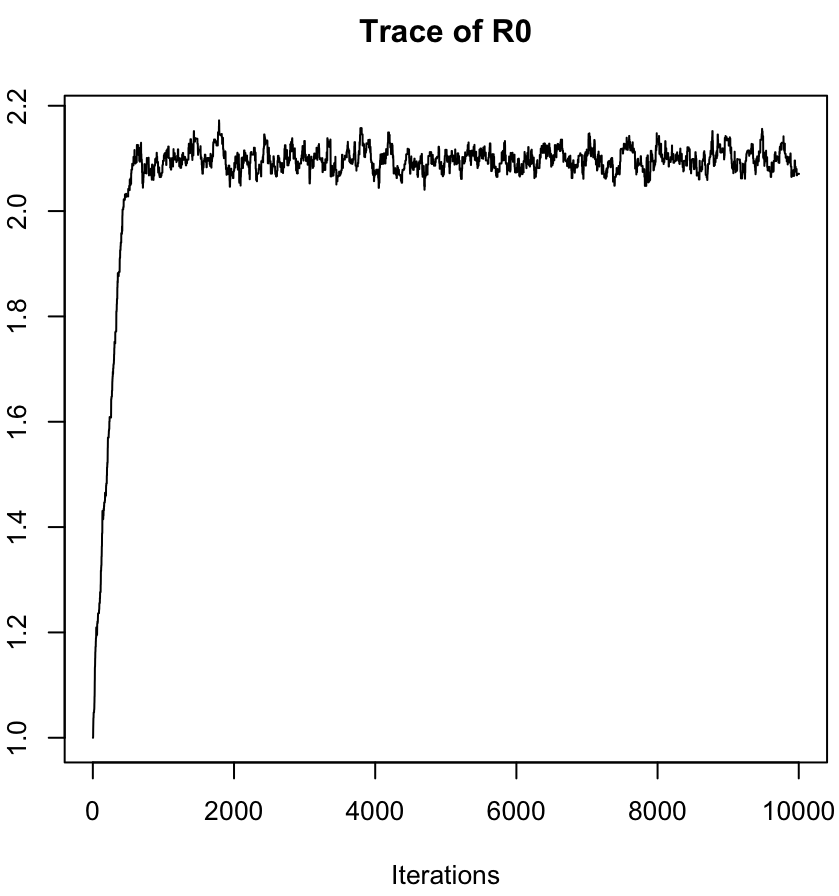
\includegraphics[width=0.45\textwidth]{trace1.png} 
         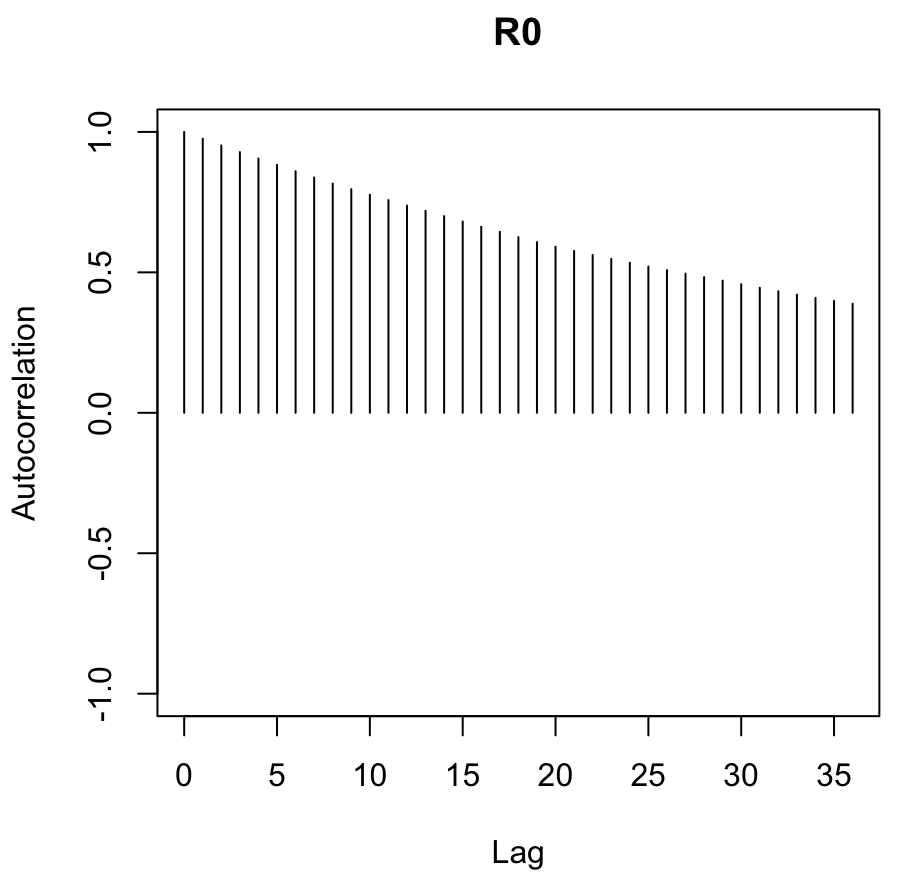
\includegraphics[width=0.5\textwidth]{index1.png}
         \caption{Exemple pour un paramètre de régression}
        \end{figure}
    \end{column}
    \end{columns}
    \end{frame}

\begin{frame}
    \frametitle{Un exemple simple pour l'\'Echantilloneur de Gibbs  }
    On simule la loi d'un vecteur gaussien 
    $
    \left(\begin{array}{l}
    {X} \\
    {Y}
    \end{array}\right) \sim N\left[\left(\begin{array}{l}
    {\mu_{1}} \\
    {\mu_{2}}
    \end{array}\right),\left(\begin{array}{ll}
    {\sigma_1^2} & {\rho} \\
    {\rho} & {\sigma_2^2}
    \end{array}\right)\right]
    $
On utilise l'échantillonneur de Gibbs en itérant:
$$
\begin{aligned}
&x_{n+1} \sim \mathcal{N}\left(\mu_{1}+\rho \frac{\sigma_{1}}{\sigma_{2}}\left(y_{n}-\mu_{2}\right), \sigma_{1}^{2}(1-\rho)\right)\\
&y_{n+1} \sim \mathcal{N}\left(\mu_{2}+\rho \frac{\sigma_{2}}{\sigma_{1}}\left(x_{n+1}-\mu_{1}\right), \sigma_{2}^{2}(1-\rho)\right)
\end{aligned}
$$ 
\end{frame}

\begin{frame}[fragile]
    \begin{lstlisting}[
        language = Python,
        basicstyle=\tiny, %or \small or \footnotesize etc.
        caption={Implémentation Python},
        captionpos=b
    ]
def sample_x_given_y(y, mean, var):
    mu = mean[0] + var[0,1] * math.sqrt(var[0, 0]) / math.sqrt(var[1, 1]) * (y - mean[1])
    var = var[0, 0] * (1 - var[1,0])
    return np.random.normal(mu, var)

def sample_y_given_x(x, mean, var):
    mu = mean[1] + var[0, 1] * math.sqrt(var[1, 1]) / math.sqrt(var[0, 0]) * (x - mean[0])
    var = var[1, 1] * (1 - var[1,0])
    return np.random.normal(mu, var)

def gibbs_sampler(mean, var, N_iter):
    samples = np.zeros((N_iter, 2))
    y = mean[1]

    for i in range(N_iter):
        x = sample_x_given_y(y, mean, var)
        y = sample_y_given_x(x, mean, var)
        samples[i, :] = [x, y]

    return samples
\end{lstlisting}
\end{frame}

\begin{frame}
    \frametitle{Simulations \normalsize
    $
    \left(\begin{array}{l}
        {\mu_{1}} \\
        {\mu_{2}}
    \end{array}\right) = 
    \left(\begin{array}{l}
        {0}\\
        {5}
    \end{array}\right)
    , \
    \sigma_1^2 = 1 ,\ \sigma_2^2 = 0.5,\ \rho = 0.6
    $}
    \begin{figure}
        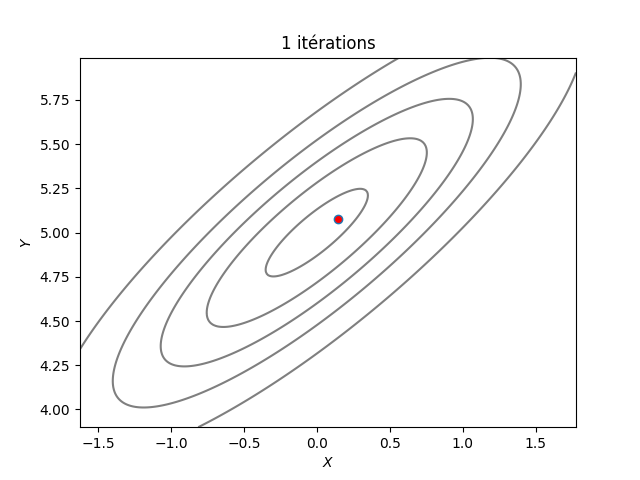
\includegraphics[width=0.45\textwidth]{../MCMC_numeric/simu/simu_1.png} 
        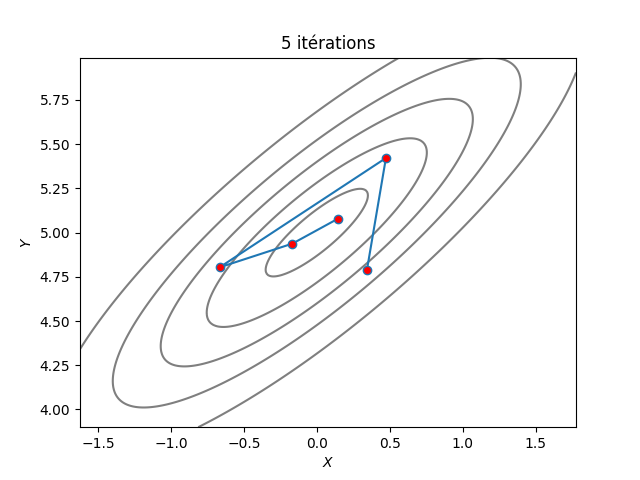
\includegraphics[width=0.45\textwidth]{../MCMC_numeric/simu/simu_5.png} 
       \end{figure}
\end{frame}

\begin{frame}
    \frametitle{Simulations \normalsize
    $
    \left(\begin{array}{l}
        {\mu_{1}} \\
        {\mu_{2}}
    \end{array}\right) = 
    \left(\begin{array}{l}
        {0}\\
        {5}
    \end{array}\right)
    , \
    \sigma_1^2 = 1 ,\ \sigma_2^2 = 0.5,\ \rho = 0.6
    $}
    \begin{figure}
        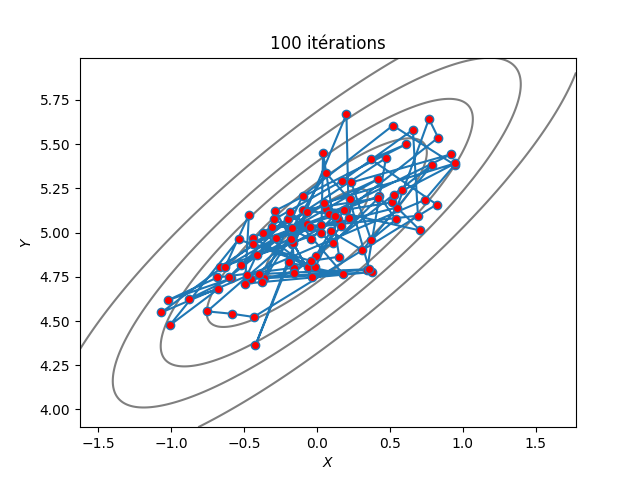
\includegraphics[width=0.45\textwidth]{../MCMC_numeric/simu/simu_100.png} 
        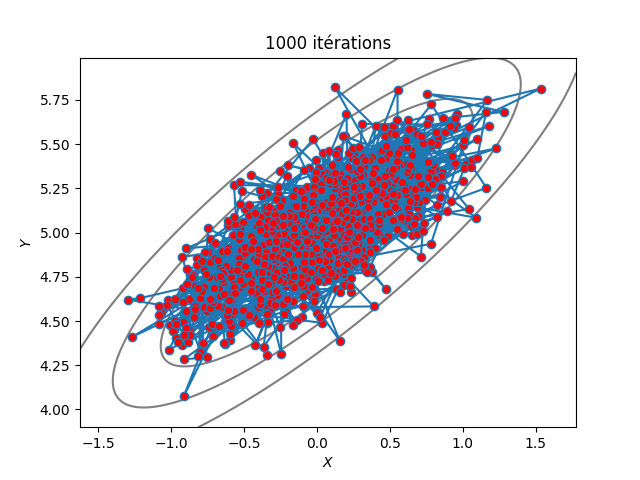
\includegraphics[width=0.45\textwidth]{../MCMC_numeric/simu/simu_1000.png} 
       \end{figure}
\end{frame}

\begin{frame}
    \frametitle{Simulations \normalsize
    $
    \left(\begin{array}{l}
        {\mu_{1}} \\
        {\mu_{2}}
    \end{array}\right) = 
    \left(\begin{array}{l}
        {0}\\
        {5}
    \end{array}\right)
    , \
    \sigma_1^2 = 1 ,\ \sigma_2^2 = 0.5,\ \rho = 0.6
    $}
    \vspace{-0.2cm}
    \begin{figure}
        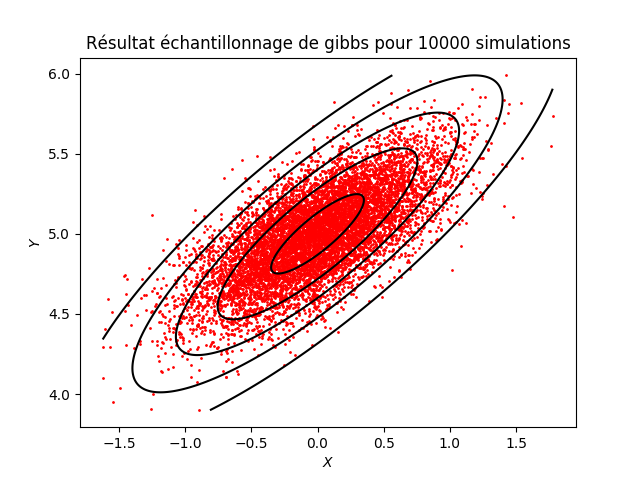
\includegraphics[width=0.65\textwidth]{../MCMC_numeric/simu/simu.png} 
       \end{figure}
\end{frame}


%.MMMMMM....MMMMMM....CCCCCCCCC..CMMMMM....MMMMMM....CCCCCCCCC..........._22222222....
%.MMMMMM....MMMMMM...CCCCCCCCCCC.CMMMMMM...MMMMMM...CCCCCCCCCCC.........._222222222...
%.MMMMMMM..MMMMMMM..CCCCCCCCCCCC.CMMMMMM..MMMMMMM..MCCCCCCCCCCC.........._2222222222..
%.MMMMMMM..MMMMMMM..CCCCC.....CC.CMMMMMM..MMMMMMM..MCCCC.....CC.........._2....22222..
%.MMMMMMMMMMMMMMMM..CCCC.........CMMMMMMM.MMMMMMM..MCCC........................22222..
%.MMMMMMMMMMMMMMMM.MCCCC.........CMMMMMMMMMMMMMMM.MMCCC........................2222...
%.MMMM.MMMMMM.MMMM.MCCCC.........CMMMMMMMMMMMMMMM.MMCCC......................222222...
%.MMMM.MMMMMM.MMMM.MCCCC.........CMMMMMMMMMM.MMMM.MMCCC.....................222222....
%.MMMM.MMMMMM.MMMM..CCCC.........CMMMM.MMMMM.MMMM..MCCC....................222222.....
%.MMMM..MMMM..MMMM..CCCCC.....CC.CMMMM.MMMM..MMMM..MCCCC.....CC...........222222......
%.MMMM..MMMM..MMMM..CCCCCCCCCCCC.CMMMM.MMMM..MMMM..MCCCCCCCCCCC.........._2222222222..
%.MMMM........MMMM...CCCCCCCCCCC.CMMMM.......MMMM...CCCCCCCCCCC.........._2222222222..
%.MMMM........MMMM....CCCCCCCCC..CMMMM.......MMMM....CCCCCCCCC..........._2222222222..
%\begin{frame}
    \frametitle{Application numérique : Une alternative à l'algorithme E-M pour le mélange de gaussiennes}
    \small
    \'Echantillon $\boldsymbol{x}=\left(\boldsymbol{x}_{1}, \ldots, \boldsymbol{x}_{N}\right)$ suivant une loi 
    $f\left(\boldsymbol{x}_{i}, \theta\right)$ 
    avec des variables latentes $\boldsymbol{z}=\left(\boldsymbol{z}_{1}, \boldsymbol{z}_{2}, \dots, \boldsymbol{z}_{n}\right)$\\
    
    \begin{columns}
        \begin{column}{0.8\textwidth}
            
            \textbf{$\rightarrow$ Algorithme E-M : } Maximisation de $L(\boldsymbol{\theta} ; \mathbf{X})=p(\mathbf{x} | \boldsymbol{\theta})=\int p(\mathbf{x}, \mathbf{z} | \boldsymbol{\theta}) d \mathbf{Z}$
            $$
            L(\mathbf{x} ; \boldsymbol{\theta})=Q\left(\boldsymbol{\theta} ; \boldsymbol{\theta}^{(c)}\right)-H\left(\boldsymbol{\theta} ; \boldsymbol{\theta}^{(c)}\right)
            $$

            $$\left\{\begin{aligned}
                Q\left(\boldsymbol{\theta} ; \boldsymbol{\theta}^{(c)}\right) &=E \left[L((\mathbf{x}, \mathbf{z}) ; \boldsymbol{\theta}) | \boldsymbol{\theta}^{(c)}\right] \\
                H\left(\boldsymbol{\theta} ; \boldsymbol{\theta}^{(c)}\right) &= E\left[\sum_{i=1}^{n} \log f\left(z_{i} | \boldsymbol{x}_{i}, \boldsymbol{\theta}\right) | \boldsymbol{\theta}^{(c)}\right]
            \end{aligned}\right.$$
            $
            \boldsymbol{\theta}^{(c+1)}=\arg \max _{\boldsymbol{\theta}}\left(Q\left(\boldsymbol{\theta}, \boldsymbol{\theta}^{(c)}\right)\right)
            $ fait tendre la suite $L\left(\mathbf{x} ; \boldsymbol{\theta}^{(c+1)}\right)$ vers un max local  
            
    \end{column}

\begin{column}{0.2\textwidth}  %%<--- here
    \vspace{-0.5cm}
    \begin{figure}
        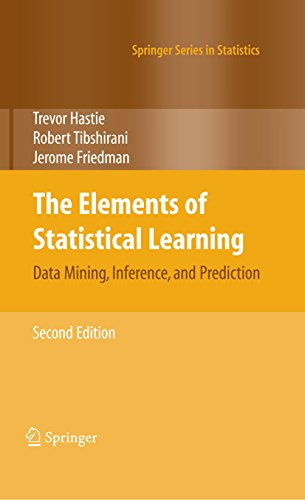
\includegraphics[width=\textwidth]{Figures/the_element.jpg}
    \end{figure}
\end{column}
\end{columns}



\end{frame}

\begin{frame}

\frametitle{Application : mélange de gaussiennes}

\vspace{-0.5cm}
\begin{columns}
    \begin{column}{0.7\textwidth}
        
        \begin{itemize}
            \item Les données $\mathbf{x}$ viennent de gaussiennes $\{ C_1,\ldots, C_M \}$ 
            %\vspace{0.5cm}
            \item $\boldsymbol{z}_{i} \in \{1,\ldots, m \}$ si un individu $i$ vient de $C_1, \ldots, C_M$
            $$ 
                \boldsymbol{x}_i |\left(\boldsymbol{z}_{i}=j\right) \sim \mathcal{N}\left(\mu_{j}, \sigma_{j}^{2}\right) \quad \mathbb{P}\left(\boldsymbol{z}_{i}=j\right)=\pi_{j} 
            $$
            $\theta=\left(\pi, \mu, \sigma^{2}\right)$ 
            \item \textbf{E-M} : maximisation de $\hat{\theta}_{\mathrm{MLE}}(x)=\underset{\theta}{\arg \max } f(x | \theta)$\\
            
            $$\ell_{\theta}(x)=\sum_{n=1}^{N} \log \left(\sum_{j=1}^{M} \pi_{j}\ \mathcal{N}_{\mu_{j}, \sigma_{j}^2}\left(x_{n}\right)\right)$$

            \item \textbf{Bayesien} estimateur $\hat{\theta}_{MMSE}(x)=E[\theta | x]$
        \end{itemize}
    \end{column}
    \begin{column}{0.3\textwidth}  %%<--- here
        \vspace{-0.5cm}
        \begin{figure}
            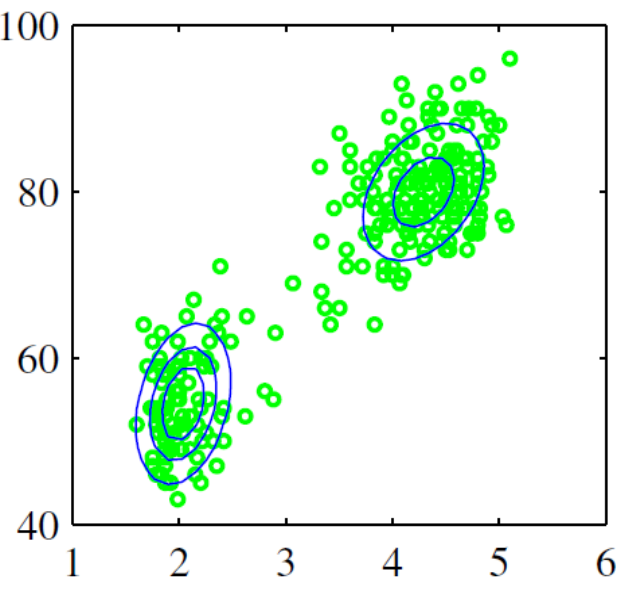
\includegraphics[width=\textwidth]{Figures/mix_gaussienne.png}
            \caption{\tiny Mélange de deux gausiennes [F. Sur, Introduction à l'apprentissage automatique]}
        \end{figure}
    \end{column}
\end{columns}

\end{frame}

\begin{frame}
    \frametitle{Application : \'Echantillonneur de Gibbs pour le mélange de 2 gaussiennes}
    Pour 2 gaussiennes:
    $\left\{\begin{aligned}
        &\boldsymbol{x}_i |\left(\boldsymbol{z}_{i}=1\right) \sim \mathcal{N}\left(\mu_{1}, \sigma_{1}^{2}\right) \quad \mathbb{P}\left(\boldsymbol{z}_{i}=1\right)=\pi_{1}\\
        &\boldsymbol{x}_i |\left(\boldsymbol{z}_{i}=2\right) \sim \mathcal{N}\left(\mu_{2}, \sigma_{2}^{2}\right) \quad \mathbb{P}\left(\boldsymbol{z}_{i}=2\right)=\pi_{2} = 1- \pi_{1}
    \end{aligned}\right.$
        \vspace{0.4cm}
        
        $\rightarrow$ On veut obtenir $\Theta = (\boldsymbol{z}, \mu) = (\boldsymbol{z_1}, \ldots,\boldsymbol{z_1},  \mu)$ \hfill($\pi, \sigma$ fixés à $\hat{\pi}, \hat{\sigma}$)
    \end{frame}

    \begin{frame}
        \frametitle{\small Application : \'Echantillonneur de Gibbs pour le mélange de 2 gaussiennes}
        \vspace{-0.5cm}
    \begin{itemize}
        \item $\Theta = (\boldsymbol{z}, \mu) = (\boldsymbol{z_1}, \ldots,\boldsymbol{z_1},  \mu)$
        \item \textcolor{beamerfooter3}{\Large $\boldsymbol{z} | \mu$} :  
        On a $p\left(\mathcal{C}_{1} | x\right)=\frac{p\left(\mathcal{C}_{1}\right) p\left(x | \mathcal{C}_{1}\right)}
        {p\left(\mathcal{C}_{1}\right) p\left(x | \mathcal{C}_{1}\right)+p\left(\mathcal{C}_{2}\right) p\left(x | \mathcal{C}_{2}\right)}$ 
        \\\vspace{0.2cm}
        Utiliser
        $\mathbb{P}\left(\boldsymbol{z}_{i}=j | \mu, \boldsymbol{x} \right)=
        { \displaystyle \frac{
            \hat{\pi}_{j}  p_{\mathcal{N}}(\boldsymbol{x}_i,\mu_{j}, \hat{\sigma}_{j})
            }{
                \hat{\pi}_{1}  p_{\mathcal{N}}(\boldsymbol{x}_i,\mu_{1}, \hat{\sigma}_{1})  +  
                \hat{\pi}_{2}  p_{\mathcal{N}}(\boldsymbol{x}_i,\mu_{2}, \hat{\sigma}_{2})
            }} \quad j \in \{ 1,2\}
            $             
        \item \textcolor{beamerfooter3}{\Large $\mu | \boldsymbol{z}$} :
        
        \begin{columns}[T]
            
            \begin{column}{0.3\textwidth}  %%<--- here
                \centering
                {\small (à priori)} \\
                \vspace{0.1cm}
                $\begin{aligned}
                    \boldsymbol{x_i} | \mu,\boldsymbol{z_i} = j & \sim \mathcal{N}\left(\mu_{j}, 1 / \hat{\tau}_j \right) \\
                    \mu_j & \sim {\mathcal{N}}\left(\mu_{0}, 1 / \tau_{0}\right) \\
                \end{aligned}$ \\
                \vspace{0.2cm}
                {\tiny $\left(\tau_j = 1 / \sigma_j^2, \ \bar{x}=\frac{1}{N} \sum_{i=0}^{N}{x_i}\right)$}
            \end{column}
            \begin{column}{0.3\textwidth}
                \centering
                {\small (à postériori)} \\
                \vspace{0.2cm}
                $\begin{aligned}
                    p(\mu_j | \boldsymbol{z}_i, \mathbf{x}) & \propto p(\boldsymbol{x} | \mu,\boldsymbol{z_i} = j) p(\mu_j)  \\
                    & \sim {\mathcal{N}}( \mu_{j_0}^{\prime}, 1 / \tau^{\prime}_{j_0}) 
                \end{aligned}$
            \end{column}
            \begin{column}{0.4\textwidth}  %%<--- here
                \centering
                {\small (= maj des coefs)} \\
                \vspace{0.1cm}
                $\begin{aligned}
                    \tau^{\prime}_{j_0} &= \tau_0 + N \hat{\tau}_j \\
                    \mu_{j_0}^{\prime} &= \frac{N\ \hat{\tau}_j\ \bar{x}+\tau_{0} \mu_{0}}{N \hat{\tau}_j+\tau_{0}} 
                \end{aligned}$
            \end{column}     
            % \begin{column}{0.14\textwidth}  %%<--- here
            %     \begin{flushleft}
                    
            %     {\tiny }
            %     \end{flushleft}
            % \end{column}     
        \end{columns}
\end{itemize}
    
\end{frame}

\begin{frame}
    \small
    \begin{exampleblock}{\'Echantilloneur de Gibbs pour une mixture gaussienne}
    \begin{enumerate}
        \item Prendre les valeurs initiales $\Theta_0 = (\boldsymbol{z}^{(0)}, \mu_{1}^{(0)}, \mu_{2}^{(0)})$, $\mu_0, \tau_0$
        \item Pour t de  à ...
            \begin{itemize}
                \item Pour $i$ de 1 à $N$ tirer \\
                {\addtolength{\leftskip}{2cm} 
                    $\boldsymbol{z}_i^{(t+1)} \in \{1, 2 \}$ avec $\mathbb{P}(\boldsymbol{z}_i^{(t+1)}=1 | \mu^{(t)}) = 
                    { \displaystyle \frac{
                    \hat{\pi}_{1}  p_{\mathcal{N}}(\boldsymbol{x}_i,\mu_{1}^{(t)}, \hat{\sigma}_{1})
                    }{
                        \hat{\pi}_{1}  p_{\mathcal{N}}(\boldsymbol{x}_i,\mu_{1}^{(t)}, \hat{\sigma}_{1})  +  
                        \hat{\pi}_{2}  p_{\mathcal{N}}(\boldsymbol{x}_i,\mu_{2}^{(t)}, \hat{\sigma}_{2})
                    }}$
                }
                \item Pour $j \in \{ 1,2\} $ \\
                Avec 
                $\tau^{\prime}_{j_0} = \tau_0 + N \hat{\tau_j} \quad \displaystyle
                \mu_{j_0}^{\prime} = \frac{N\ \hat{\tau_j}\ \bar{x}+\tau_{0} \mu_{0}}{N \hat{\tau_j}+\tau_{0}} 
                $ \\
                Tirer $\mu_{j}^{(t+1)}\ \boldsymbol{z} \sim \mathcal{N}\left(\mu_{j_0}^{\prime}, 1 / \tau^{\prime}_{j_0}\right)$
            \end{itemize}
    \end{enumerate}
   
\end{exampleblock}
\end{frame}

\begin{frame}[fragile]
    %\frametitle{\tiny Implémentation sous R}
    \vspace{-0.2cm}
    \begin{columns}
        \begin{column}{0.5\textwidth}
            
            \begin{lstlisting}[
                basicstyle=\fontsize{5}{5}\selectfont\ttfamily, %or \small or \footnotesize etc.
                captionpos=b,
                numbers = none
            ]
Z_given_mu <- function(X,Z,mu,pi_1){
    # Z variables latentes
    
    remove_i <- (c(1:length(X)) !=i) # enleve variable i
    estimate_sigma_1 <- sd(X[(remove_i & Z == 1)]) # classe 1
    estimate_sigma_2 <- sd(X[(remove_i & Z == 2)]) # classe 2 
                    
    for (i in 1:length(Z)){
                    
        proba1 <- pi_1 * dnorm(X[i],mu[1],estimate_sigma_1) / 
            (pi_1 * dnorm(X[i],mu[1],estimate_sigma_1) + 
            (1-pi_1) * dnorm(X[i],mu[2],estimate_sigma_2))

        Z[i] = sample(1:2, size=1,prob=c(proba1, 1-proba1),
            replace=TRUE)
    }
    return(Z)
}
        \end{lstlisting}
            
        \end{column}
        \begin{column}{0.5\textwidth}  %%<--- here
            
            \begin{lstlisting}[
                basicstyle=\fontsize{5}{5}\selectfont\ttfamily, %or \small or \footnotesize etc.
                captionpos=b,
                numbers = none
            ]
mu_given_Z = function(X, Z, mu_prior){
    # Z variables latentes  
    # mu_prior contient parametres loi a priori de mu

    mu = rep(0,2) ; sigma = rep(0,2)
        
    for(j in 1:2){
        
        sample_j_size = sum(Z==j) 
        sample_j_mean = mean(X[Z==j])
        sigma[j] = sd(X[Z==j]) ; precision_j = 1 / sigma[j]^2
        
        precision_post = sample_j_size * precision_j + 
            mu_prior$precision
        
            mean_post = (sample_j_mean * sample_j_size * 
            precision_j + mu_prior$mean * 
            mu_prior$precision ) / precision_post
        
        mu[j] = rnorm(1,mean_post,sqrt(1/precision_post)) # on tire mu selon la loi normale a posteriori
    }
    return(list(mu = mu, sigma = sigma))
    }
        \end{lstlisting}
    \end{column}
\end{columns}
\vspace{-0.3cm}
\begin{lstlisting}[
    basicstyle=\fontsize{5}{5}\selectfont\ttfamily, %or \small or \footnotesize etc.
    captionpos=b,
    caption={\tiny Implémentation en R},
    numbers = none
]
echantillonneur_gibbs <- function(X,N_simu){
    # X sont les donnees
    # initalisation
    .
    .
    
    for (k in 1:N_simu){ 
        
        Z <- Z_given_mu(X,Z,mu,pi_1) ; param_post <- mu_given_Z(X, Z, mu_prior)
        mu = param_post$mu
    .
    .
    .
    }
    return(list(Z, mu_1, mu_2))
}     
\end{lstlisting}
\end{frame}

\begin{frame}
    \frametitle{Simulations} \hfill \small Données : on gènere équiprobablement 1000 points à partir de 2 gaussiennes $\mathcal{N}\left(-2, 1\right), \mathcal{N}\left(-3, 0.5\right)$
    
    \centering
   
            
            \begin{figure}
                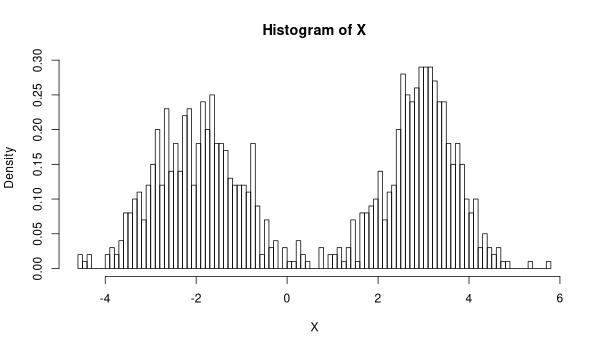
\includegraphics[width=0.55\textwidth]{../MCMC_numeric/simu_gaussian/data.png} 
            \end{figure}
   
    \vspace{-0.2cm}
    
    On prend à priori $\mu \sim \mathcal{N}\left(0, 4\right)$
\end{frame}

\begin{frame}
    \frametitle{Simulations} 
    \centering
    \small Pour 1000 itérations
    \vspace{0cm}
    \begin{columns}
        \begin{column}{0.8\textwidth}
            \begin{figure}
                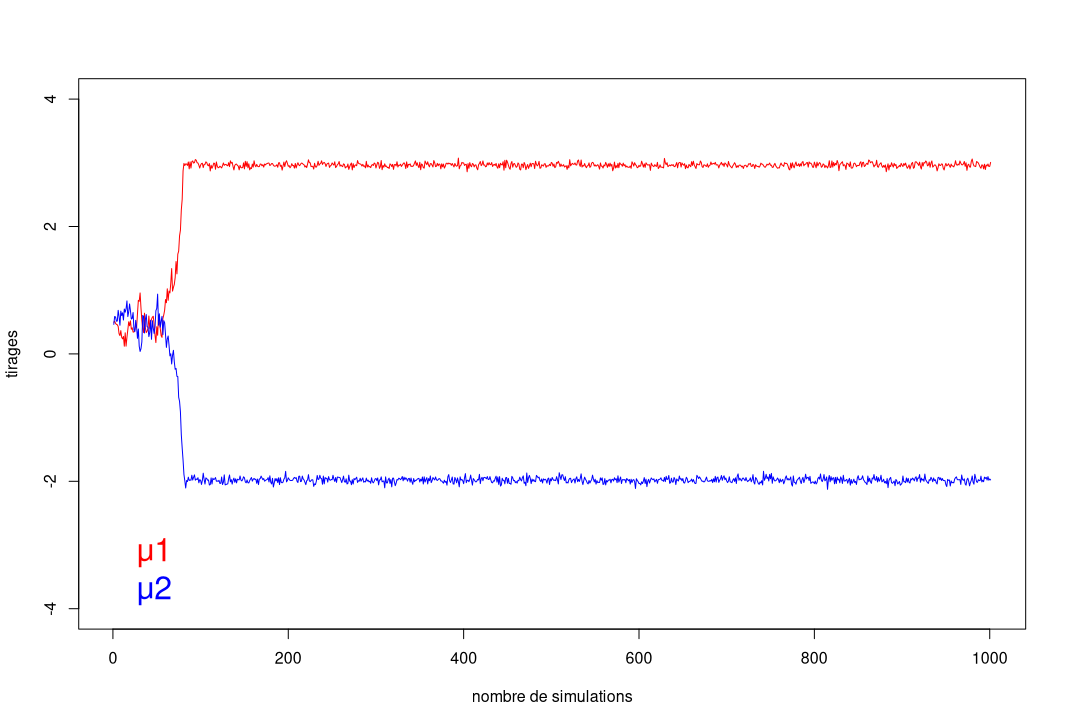
\includegraphics[width=0.8\textwidth]{../MCMC_numeric/simu_gaussian/mu.png} 
            \end{figure}
            
        \end{column}
        \begin{column}{0.2\textwidth}
            \centering
            $\rightarrow$ \textit{burn-in} de 100
        \end{column}
    \end{columns}
    \end{frame}


\begin{frame}
    \frametitle{Simulations : diagnostic de $\mu$ avec le package coda}
    \centering
    \vspace{-0.2cm}
    \begin{columns}
        \begin{column}{0.5\textwidth}
            
            \begin{figure}
                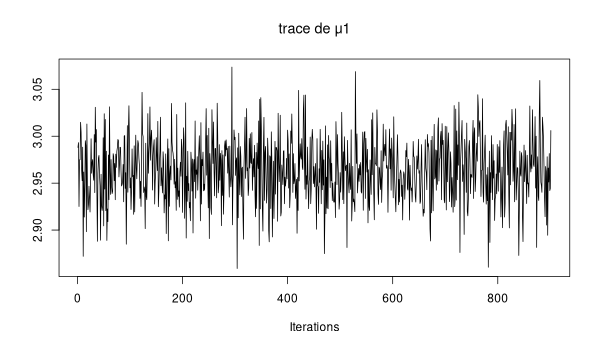
\includegraphics[width=\textwidth]{../MCMC_numeric/simu_gaussian/mu_plot_trac.png} 
            \end{figure}
        \end{column}
        \begin{column}{0.5\textwidth}

            \begin{figure}
                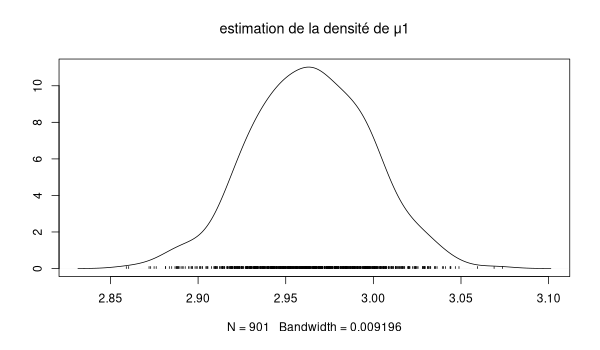
\includegraphics[width=\textwidth]{../MCMC_numeric/simu_gaussian/mu_plot_dens.png} 
            \end{figure}
        \end{column}
    \end{columns}
    (sans le \textit{burn-in})
\end{frame}
\begin{frame}
    \frametitle{Simulations : diagnostic de $\mu$ avec le package coda}

    \begin{table}[]
        \begin{tabular}{ccccc}
        \hline
        \multicolumn{1}{|l|}{variable} & \multicolumn{1}{l|}{moyenne} & \multicolumn{1}{l|}{95\% CI lower} & \multicolumn{1}{l|}{95\% CI upper} & \multicolumn{1}{l|}{vraie valeur} \\ \hline
        $\mu_1$                        & 2.963882                     & 2.899498                           & 3.032716                           & 3                                 \\ \hline
        $\mu_2$                        & -1.981757                    & -2.061083                          & -1.902244                          & -2                                \\ \hline
        \end{tabular}
        \end{table}
\end{frame}







\section{Approche bayésienne pour la modélisation des series temporelles}

% //.....................................................................................................................
% //................................................................... iii..............................................
% //.BBBBBBBBBB........................................................ iii................tttt..........................
% //.BBBBBBBBBBB....................................................... iii................tttt..........................
% //.BBBBBBBBBBB...........................................................................tttt...........r..............
% //.BBBBB..BBBB...aaaaaaaaa.aayy....yyyy..eeeeeeee....ssssssss........ iii...nnnnnnnnn..nnttttttt.trrrrrrr..oooooooo....
% //.BBBBB.BBBBB...aaaaaaaaa.aayyy..yyyyy.yeeeeeeeee..essssssss........ iii...nnnnnnnnnn.nnttttttt.trrrrrrr.rooooooooo...
% //.BBBBBBBBBBB...aaaaaaaaaa.ayyy..yyyy..yeeeeeeeee..essssssss........ iii...nnnnnnnnnn.nnttttttt.trrrrrrrrrooooooooo...
% //.BBBBBBBBBBB...aaaaaaaaaa.ayyyy.yyyy.yyeee..eeeee.esssss........... iii...nnnn..nnnn...tttt....trrrr...rrooo..ooooo..
% //.BBBBBBBBBBBB.Baaaaaaaaaa..yyyyyyyyy.yyeeeeeeeeee.essssssss........ iii...nnnn..nnnn...tttt....trrr....rroo...ooooo..
% //.BBBBB..BBBBB.Baaaaa.aaaa..yyyyyyyy..yyeeeeeeeeee..ssssssss........ iii...nnnn..nnnn...tttt....trrr....rroo...ooooo..
% //.BBBBB..BBBBB.Baaa..aaaaa...yyyyyyy..yyeee.....e......ssssss....... iii...nnnn..nnnn...tttt....trrr....rrooo..ooooo..
% //.BBBBBBBBBBBB.Baaaaaaaaaa...yyyyyy....yeeeeeeeee..esssssssss....... iii...nnnn..nnnn...ttttttt.trrr....rrooooooooo...
% //.BBBBBBBBBBBB.Baaaaaaaaaa...yyyyyy....yeeeeeeeee..essssssss........ iii...nnnn..nnnn...ttttttt.trrr.....rooooooooo...
% //.BBBBBBBBBBB...aaaaaaaaaa....yyyyy.....eeeeeeeee..essssssss........ iii...nnnn..nnnn...ttttttt.trrr......oooooooo....
% //.............................yyyy....................................................................................
% //...........................yyyyyy....................................................................................
% //...........................yyyyy.....................................................................................
% //...........................yyyyy.....................................................................................

\begin{frame}
    \frametitle{Approche bayésinne pour la modélisation des séries temporelles}
    \setbeamertemplate{itemize items}[triangle]
    \begin{itemize}
        \item Les modèle espace-états      
    \end{itemize}
    \setbeamertemplate{itemize items}[square]
    \bgroup
    \def\arraystretch{1.2}
\begin{table}[]
    \begin{tabular}{lll}
                                                                                               &                                                                         & bruit blanc gaussien       \\ \hline
    \rowcolor[HTML]{96FFFB} 
    \multicolumn{1}{l|}{\cellcolor[HTML]{96FFFB}{\color[HTML]{333333} equation d'observation}} & \multicolumn{1}{l|}{\cellcolor[HTML]{96FFFB}{\color[HTML]{333333} $y_{t} =Z_{t}^{T} \alpha_{t}+\epsilon_{t}$}} & {\color[HTML]{333333} $\epsilon_{t} \sim \mathcal{}{N}\left(0, H_{t}\right)$} \\ \hline
    \rowcolor[HTML]{FFFFC7} 
    \multicolumn{1}{l|}{\cellcolor[HTML]{FFFFC7}{\color[HTML]{333333} equation de transition}} & \multicolumn{1}{l|}{\cellcolor[HTML]{FFFFC7}{\color[HTML]{333333} $\alpha_{t+1} =T_{t} \alpha_{t}+R_{t}\eta_{t} $}} & {\color[HTML]{333333} $ \eta_{t} \sim \mathcal{}{N}\left(0, Q_{t}\right)$} \\
                                                                                               &                                                                         &                           
    \end{tabular}
    \end{table}
    \egroup
    \vspace{-1cm}
        \begin{columns}
        \begin{column}{0.5\textwidth}
            
            \begin{itemize}
                \item $y_t$ obervations
                \item $\alpha_t$ variables d'états / latentes / cachées
                \item $Z_t$ matrice de mesure
                \item $T_t$ matrice de transitions
            \end{itemize}
        \end{column}
        
        \begin{column}{0.5\textwidth}
            \begin{figure}
                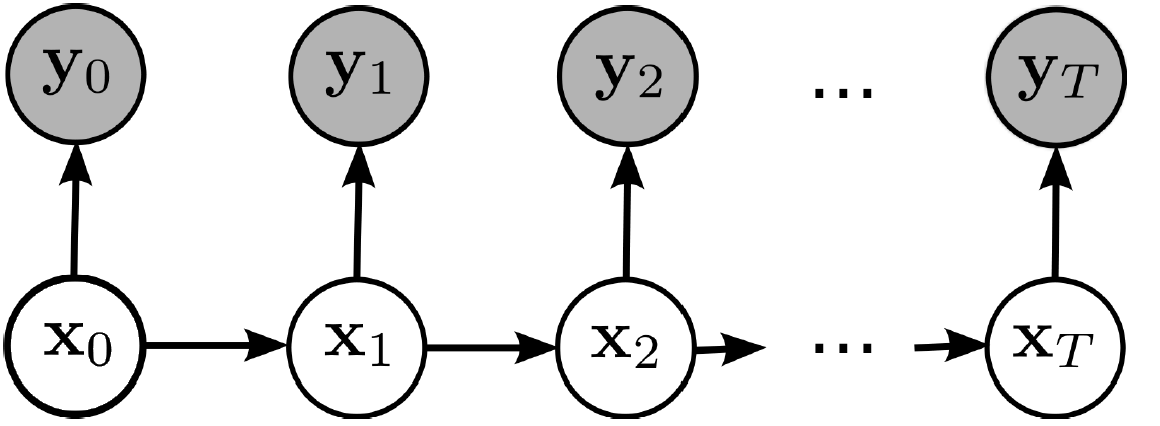
\includegraphics[width=\textwidth]{Figures/hmc.png}
                \caption{[researchgate.net]}
            \end{figure}
        \end{column}
    \end{columns}
\end{frame}

\begin{frame}
    \frametitle{Approche bayésinne pour la modélisation des séries temporelles}
    
    $\rightarrow$ Bayesian structural time series (BSTS) 
    \bgroup
    \def\arraystretch{1.5}
\begin{table}[]
    \begin{tabular}{lll}
        &                                                                         & bruit blanc gaussien       \\ \hline
\rowcolor[HTML]{96FFFB} 
\multicolumn{1}{l|}{\cellcolor[HTML]{96FFFB}{\color[HTML]{333333} observation}} & \multicolumn{1}{l|}{\cellcolor[HTML]{96FFFB}{\color[HTML]{333333} $y_{t}=\mu_{t}+\beta^{T} x_{t}+\tau_t +\varepsilon_{t}$}}  & {\color[HTML]{333333} $\varepsilon_{t} \sim N\left(0, \sigma_{\varepsilon}^{2}\right)$} \\ \hline
\multicolumn{1}{l|}{regression}                                                 & \multicolumn{1}{l|}{${\beta^{T} x_{t}}$}                                 &                      \\ \hline
\multicolumn{1}{l|}{tendance + marche aléatoire}                                & \multicolumn{1}{l|}{${\mu_{t}=\mu_{t-1}+\delta_{t-1}+u_{t}}$}            & $u_{t} \sim N\left(0, \sigma_{u}^{2}\right)$                        \\ \hline
\multicolumn{1}{l|}{marche aléatoire}                                           & \multicolumn{1}{l|}{$\delta_{t}=\delta_{t-1}+v_{t}$}                     & $v_{t} \sim N\left(0, \sigma_{v}^{2}\right)$                        \\ \hline
\multicolumn{1}{l|}{sainsonnalité}                                              & \multicolumn{1}{l|}{$\tau_{t}=-\sum_{s=1}^{s-1} \tau_{t-s}+w_{t}$}       & $w_{t} \sim N\left(0, \sigma_{w}^{2}\right)$                       
\end{tabular}
\end{table}
\egroup
\end{frame}


\begin{frame}
    \frametitle{}
    $\rightarrow$ Bayesian structural time series (BSTS)
    \bgroup
    \def\arraystretch{1.5}
    \begin{table}[]
        \begin{tabular}{l|l|l}
        \rowcolor[HTML]{34CDF9} 
        \multicolumn{1}{l|}{\cellcolor[HTML]{34CDF9}{\color[HTML]{333333} observation}}  & \multicolumn{1}{l|}{\cellcolor[HTML]{34CDF9}{\color[HTML]{333333} $y_{t} =Z_{t}^{T} \alpha_{t}+\epsilon_{t}$}} & {\color[HTML]{333333} $\epsilon_{t} \sim \mathcal{}{N}\left(0, H_{t}\right)$} \\ \hline  
                & \multicolumn{1}{c|}{$Z_t^T$}        & \multicolumn{1}{c|}{$\alpha_t^T$} \\
                    & \multicolumn{1}{c|}{$(\begin{array}{lll}{1} & {0} & {\beta^{T} \mathbf{x}_{t}}\end{array})$}              & \multicolumn{1}{c|}{$\left(\begin{array}{lll}{\mu_{t}} & {\delta_{t}} & {1}\end{array}\right)^{T}$}      \\ \hline
        \rowcolor[HTML]{34CDF9} 
        \multicolumn{1}{l|}{\cellcolor[HTML]{34CDF9}{\color[HTML]{333333} equation de transition}} & \multicolumn{1}{l|}{\cellcolor[HTML]{34CDF9}{\color[HTML]{333333} $\alpha_{t+1} =T_{t} \alpha_{t}+R_{t}\eta_{t} $}} & {\color[HTML]{333333} $ \eta_{t} \sim \mathcal{}{N}\left(0, Q_{t}\right)$} \\
        \multicolumn{1}{c|}{$\alpha_t$}  & \multicolumn{1}{c|}{$T_t$} & \multicolumn{1}{c|}{$N_t \eta_t$}         \\
    \multicolumn{1}{c|}{$\left(\begin{array}{c}{\mu_{t}} \\ {\delta_{t}} \\ {1}\end{array}\right)$}        & \multicolumn{1}{c|}{$\left(\begin{array}{lll}{1} & {1} & {0} \\ {0} & {1} & {0} \\ {0} & {0} & {1}\end{array}\right)$}           & \multicolumn{1}{c|}{$\left(\begin{array}{c}{u_{t}} \\ {v_{t}} \\ {w_t}\end{array}\right)$}       
        \end{tabular}
        \end{table}
        \egroup

        $\rightarrow$ estimation des paramètres
\end{frame}



    




\begin{frame}
    \frametitle{Loi à postériori états cachés $\alpha_t$ : Le filtre de Kalman }
    \centering
    Itérations sur l'estimation $p(\alpha_{t} | y_{1: t}) \sim \mathcal{N}(\hat{\alpha}_{t}, P_t)$
    \begin{figure}
        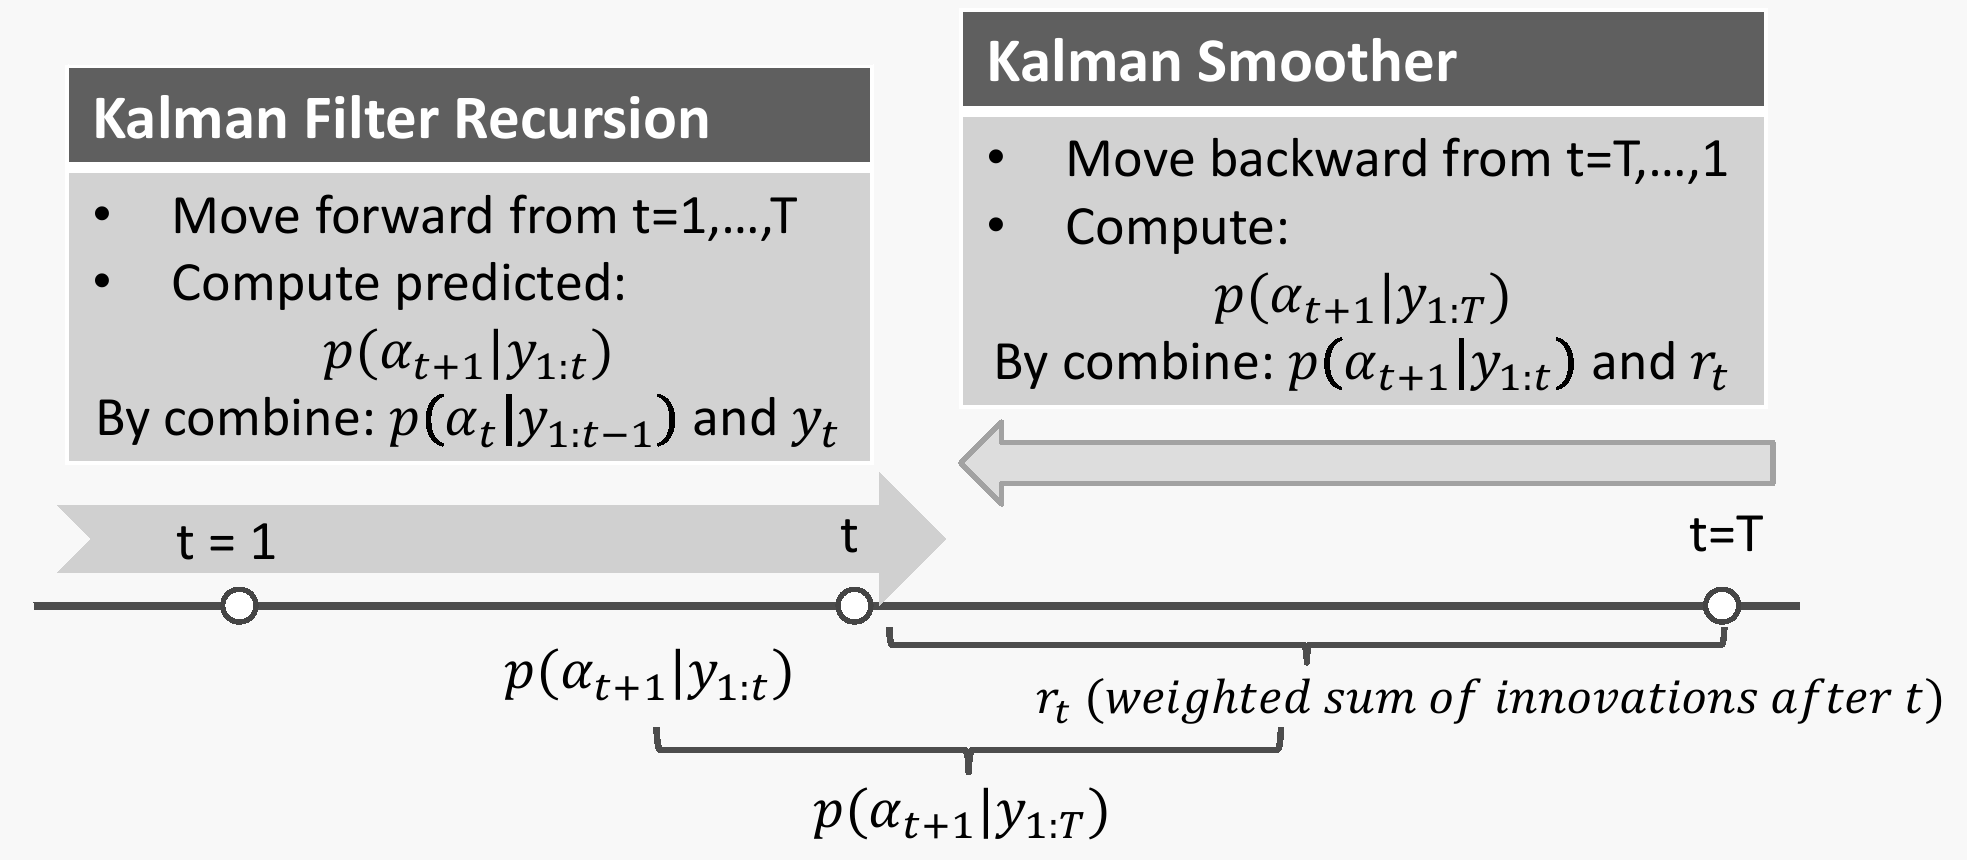
\includegraphics[width=0.8\textwidth]{Figures/kalman_filter.png}
        \caption{[github : anhdanggit/nowcasting-google-queries/]}
    \end{figure}
    
    
\end{frame}

\begin{frame}
    \frametitle{Loi à postériori de $\beta$: \textit{spike-and-slab prior}}
    \vspace{-1cm}
    \begin{columns}
        \begin{column}{0.8\textwidth}
            \vspace{-1cm}
            \begin{itemize}
                \item On prend la partie regression $y_{t}^{*}=y_{t}-\mu_{t}$
                \item On utilise pour $\beta$ une distribution à priori \textit{spike-and-slab}:
            \end{itemize}
            
        \end{column}
        \begin{column}{0.2\textwidth}

            \begin{figure}
                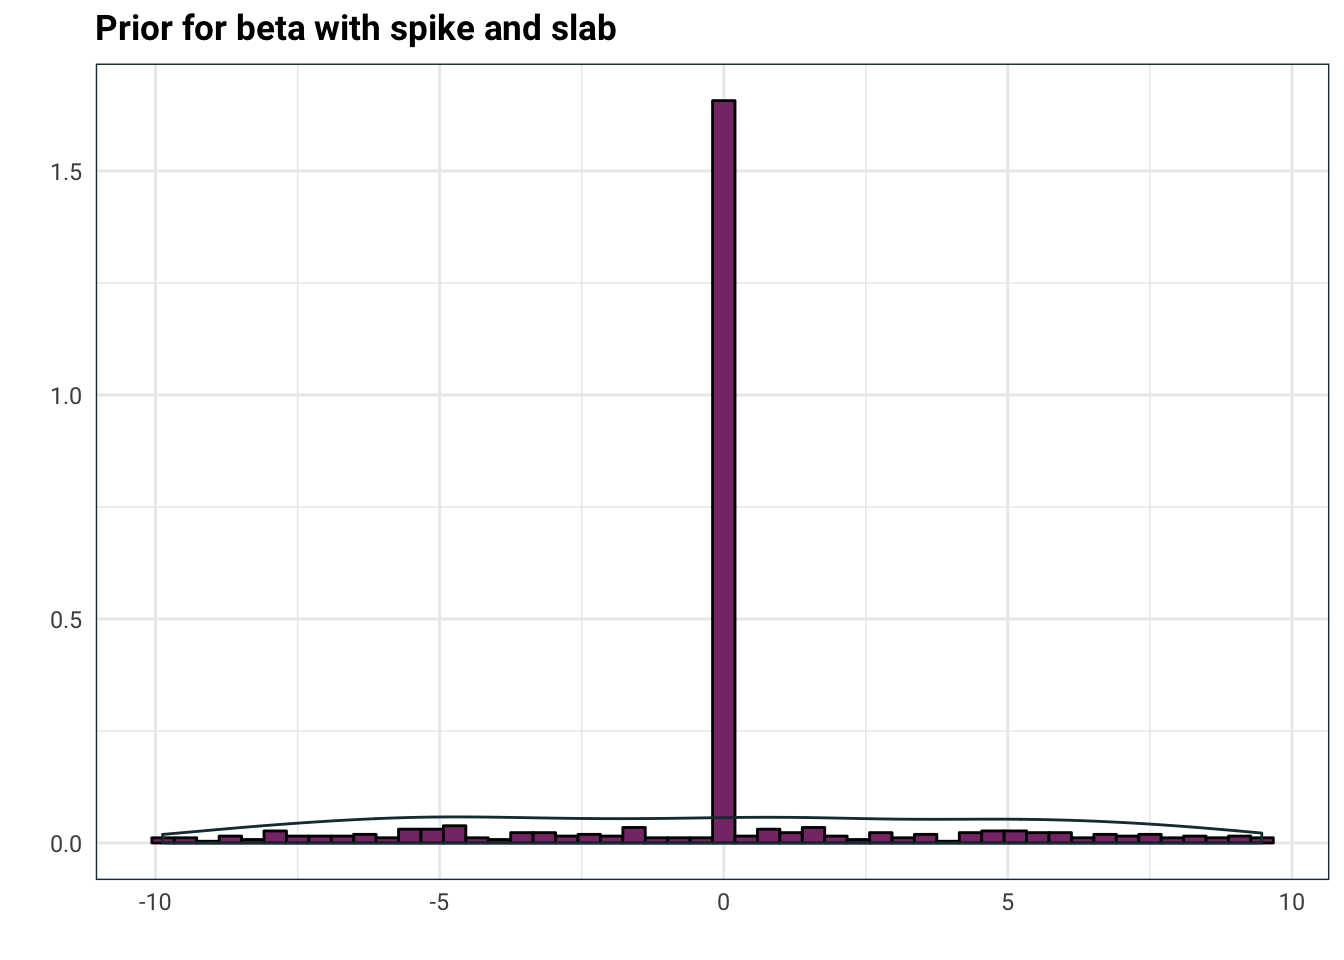
\includegraphics[width=\textwidth]{Figures/pike.png}
                \caption{[batisengul.co.uk]}
            \end{figure}
        
        \end{column}
\end{columns}
\vspace{-1.5cm}
       \setbeamertemplate{itemize items}[triangle]
     
           
    
        \begin{itemize}
            \item  $\displaystyle p(\gamma)=\prod_{k=1}^{N} \pi^{\gamma_k}(1-\pi)^{1-\gamma_k}$, $\gamma_k \in \{0,1 \}$ {\small $N = Card(\mathbf{x})$} 
            \item \'A priori : $p\left(\beta, \gamma, \sigma_{\varepsilon}^{2}\right)=p\left(\beta_{\gamma} | \gamma, \sigma_{\varepsilon}^{2}\right) p\left(\sigma_{\varepsilon}^{2} | \gamma\right) p(\gamma)$ 
            \item $
                \beta_{\gamma}\left|\sigma_{\epsilon}^{2}, \gamma \sim \mathcal{N}\left(b_{\gamma},
                \sigma_{\epsilon}^{2}\left(\Omega_{\gamma}^{-1}\right)^{-1}\right) \quad \sigma_{\epsilon}^{2}\right| \gamma \sim IG\left(\frac{\nu}{2}, \frac{s s}{2}\right)
                $ \\ \vspace{0.2cm}
                {\centering \tiny
                papramètres à priori : $v$ nombre de paramètres,$\quad$ $\frac{s s}{v}=\left(1-R^{2}\right) s_{y}^{2}$, $\quad$         $\Omega^{-1} \propto X^{T} X$ }
        \end{itemize}
    
        \setbeamertemplate{itemize items}[square]
   
    \begin{itemize}
        
        \item On utilise les propriété des lois conjugé pour obtenir les loi à postériori \\ \vspace{0.1cm}
        {\centering
        $\beta_{\gamma} | \sigma_{\epsilon}, \gamma, \mathbf{y}^{*} \quad \quad \gamma_\epsilon^{2} | \gamma, \mathbf{y}^{*} \quad \quad \gamma | \mathbf{y}^{*}$}
        \item Intérêt de la \textit{spkie-and-slab}
    \end{itemize}

\end{frame}

\begin{frame}
    \small
\begin{exampleblock}{\'Echantilloneur de Gibbs pour BSTS : SSVS algorithm}
    \setbeamertemplate{itemize items}[triangle]
    $\Theta=\left(\gamma, \beta, \sigma_{\varepsilon}^{2}, \sigma_{v}^{2}, \sigma_{u}^{2}\right)$
    \begin{itemize}
    \item Choisir paramètres à priori $v$, $R^2$, $s_y^2$
    \item Tirer $\gamma, \beta, \sigma_{\varepsilon}^{2}, \sigma_{v}^{2}, \sigma_{u}^{2}$ \hfill $\sigma_u^2$,$\sigma_u^2$,$\sigma_w^2$ sont tiré selon la loi $. | \gamma \sim I G\left(\frac{\nu}{2}, \frac{s s}{2}\right)$
    \end{itemize}
Sur $1, \ldots, M$:
\begin{enumerate}
\item Après application du filtre de Kalman, on tire les états latents $\alpha$ depuis $p\left(\alpha | y, \gamma, \beta, \sigma_{\varepsilon}^{2}, \sigma_{v}^{2}, \sigma_{u}^{2}\right)$
\item On tire $\sigma_u^2$ et $\sigma_v^2$ selon $p\left(\frac{1}{\sigma_{u}^{2}}, \frac{1}{\sigma_{v}^{2}} | y, \alpha, \beta, \sigma_{\varepsilon}^{2}\right)$
\item On tire $\beta$ et $\sigma_\epsilon^2$ selon $p\left(\beta, \sigma_{\varepsilon}^{2} | y, \alpha, \sigma_{u}^{2}, \sigma_{v}^{2}\right)$
\end{enumerate}

On prend comme modèle la moyenne des tirages $\left(\Theta^m, \ldots, \Theta^M\right)$

\end{exampleblock}

\end{frame}




























\begin{frame}
    \normalsize
    \frametitle{Conclusion}

    \begin{itemize}
        \item Auteur prèfère mettre incertitude dans la prior que sur l'estimation des coéfficientss
    \end{itemize}
\end{frame}

\breakingframe{
\begin{textblock*}{13cm}(3.5cm,4cm)
    
\Huge\textbf{\textcolor{black}{Merci de votre attention}}
\end{textblock*}
}


% //.TTTTTTTTTTTTTEEEEEEEEEEE..MMMMM.....MMMMM...PPPPPPPPPP...LLLL..........AAAAAA..AAATTTTTTTTTT.TEEEEEEEEE..
% //.TTTTTTTTTTTTTEEEEEEEEEEE..MMMMMM...MMMMMM...PPPPPPPPPPP..LLLL..........AAAAAA..AAATTTTTTTTTT.TEEEEEEEEE..
% //.TTTTTTTTTTTTTEEEEEEEEEEE..MMMMMM...MMMMMM...PPPPPPPPPPP..LLLL..........AAAAAAA.AAATTTTTTTTTT.TEEEEEEEEE..
% //.....TTTT.....EEEEE........MMMMMMM.MMMMMMM...PPPP...PPPP..LLLL.........AAAAAAAA......TTTT.....TEEEE.......
% //.....TTTT.....EEEEE........MMMMMMM.MMMMMMM...PPPP...PPPP..LLLL.........AAAAAAAAA.....TTTT.....TEEEE.......
% //.....TTTT.....EEEEEEEEEE...MMMMMMMMMMMMMMM...PPPP.PPPPPP..LLLL.........AAAAAAAAA.....TTTT.....TEEEEEEEEE..
% //.....TTTT.....EEEEEEEEEE...MMMMMMMMMMMMMMM...PPPPPPPPPPP..LLLL........AAAAA.AAAA.....TTTT.....TEEEEEEEEE..
% //.....TTTT.....EEEEEEEEEE...MMMMMMMMMM.MMMM...PPPPPPPPPP...LLLL........AAAA..AAAAA....TTTT.....TEEEEEEEEE..
% //.....TTTT.....EEEEE........MMMM.MMMMM.MMMM...PPPPPPPPP....LLLL.......AAAAAAAAAAAA....TTTT.....TEEEE.......
% //.....TTTT.....EEEEE........MMMM.MMMMM.MMMM...PPPP.........LLLL.......AAAAAAAAAAAA....TTTT.....TEEEE.......
% //.....TTTT.....EEEEEEEEEEE..MMMM..MMM..MMMM...PPPP.........LLLLLLLLLL.AAAAAAAAAAAAA...TTTT.....TEEEEEEEEE..
% //.....TTTT.....EEEEEEEEEEE..MMMM.......MMMM...PPPP.........LLLLLLLLLLLAAAA.....AAAA...TTTT.....TEEEEEEEEE..
% //.....TTTT.....EEEEEEEEEEE..MMMM.......MMMM...PPPP.........LLLLLLLLLLLAAAA.....AAAAA..TTTT.....TEEEEEEEEE..

% \section{exemple Utilisation template}

% \begin{frame}
% \frametitle{Blocky block}
% \begin{block}{Just a Block}
% \lipsum[1]
% \end{block}
% \end{frame}

% \begin{frame}
% \frametitle{Blocky block}
% \begin{exampleblock}{Example Block}
% \lipsum[1]
% \end{exampleblock}
% \end{frame}

% \begin{frame}
% \frametitle{Blocky block}
% \begin{alertblock}{Alert Block}
% \lipsum[1]
% \end{alertblock}
% \end{frame}

% \subsection{Frames breaker}
% \begin{frame}[fragile]
% \frametitle{How to use frame-breakings?}
%     In this template, and only this, I defined a "breakingframe" template frame that should not hold any useful information. The background of this frame is pinkish solid and it is not countable as a separate frame. You can use this as a transitioning page between different topics or for any funny funky stuff to release the tense of the poor audience during your presentation.
%     \vspace{10pt}
%     \begin{lstlisting}
%         \breakingframe{
%             Put your contents here, such as images, text ..etc. Be as silly as possible .. or not!
%         }
%     \end{lstlisting}
%     \vspace{10pt}
%     Look at the next slide, in code, as an example!
% \end{frame}

% \begin{frame}[t]{Motivation: \textcolor{myviolet}{{\textbf{Q1}}}}\vspace{10pt}
%     \begin{textblock*}{13cm}(1.7cm,2.7cm)
%     \begin{enumerate}[<+->]
%     \setlength\itemsep{10pt}
%         \item Stone masonry walls are usually not homogeneous through the thickness
%         \item Leaf-separation effects on the strength capacity
%         \item In-plane and out-of-plane behaviours interaction
%         \item Internal cracking onsets and 3D crack paths (cannot be captured experimentally)
%     \end{enumerate}
%     \end{textblock*}
% \end{frame}

% \subsection{Methodology}
% \begin{frame}[t]{The study main phases}\vspace{10pt}
%     \begin{textblock*}{13cm}(3.8cm,0.7cm)
%         
\includegraphics[height = 0.6\textwidth]{univ.png}
%     \end{textblock*}
% \end{frame}


% \breakingframe{
% \begin{textblock*}{13cm}(3.5cm,4cm)
% \Huge\textbf{\textcolor{black}{How to arrange stones?}}
% \end{textblock*}
% }

% \begin{frame}[t]{Objective function}\vspace{1pt}
% \begin{columns}
% \begin{column}{0.49\textwidth}
% \begin{overprint}
% \onslide<1->\begin{block}{Packing objective}
%     \begin{equation*}
%         \text{Minimize}~F(\vec{X_i})_{i}~=~\mid\mid \vec{S}_{i} - \vec{S}_{i-1} \mid\mid
%     \end{equation*}
%     \begin{equation*}
%         Fitness\Big(F(\vec{X_i})\Big)_{i} = F(\vec{X_i})_{i}(1 + \xi_{1} P_A)^{\xi_{2}}
%     \end{equation*}
% \end{block}
% \end{overprint}
% \end{column}
% \end{columns}
% \begin{textblock*}{3.2cm}(12.5cm,1.5cm)
%     \tiny{
%     \begin{itemize}
%         \item $S_{i}, S_{i-1}$: locations of $i$ and $i-1$ stones
%         \item $\xi_{1}$: penalty multiplier
%         \item $\xi_{2}$: penalty exponent
%         \item $P_{A}$: penalties summation
%     \end{itemize}
%     }
% \end{textblock*}
% \begin{textblock*}{3cm}(12.5cm,1.55cm)
%     %\includegraphics[height = 0.6\linewidth]{brace.pdf}
% \end{textblock*}
% \end{frame}

% % -----------------------References
% % Thank you slide should be here
% \breakingframe{
% \begin{textblock*}{10cm}(3.2cm,4cm)
% \Huge\textbf{\textcolor{black}{Merci de votre attention}}
% \end{textblock*}
% }
% -----------------------References
% \section{Bibliography}
% % \begin{frame}[allowframebreaks]{\\References}\vspace{4pt}
% \begin{frame}{References}\vspace{4pt}
% %\tiny{\printbibliography}
% \end{frame}
% \normalsize

\end{document}β
